I trained a Tree-Augmented Na\"{i}ve Bayes network on 20,950 training cases [figure \ref{fig:mass_net}] and measured the incompleteness score on 3,695 test cases, results are shown in figure \ref{fig:incompleteness_score_hist_all}. The resulting incompleteness scores were heavily right-skewed distributions. 83\% of the incompleteness scores were equal to zero, meaning no new information would have changed the follow-up decision. Hence, both the median and mode incompleteness scores were zero. The mean incompleteness score was 0.021.

\begin{figure}[h]
	\centering
	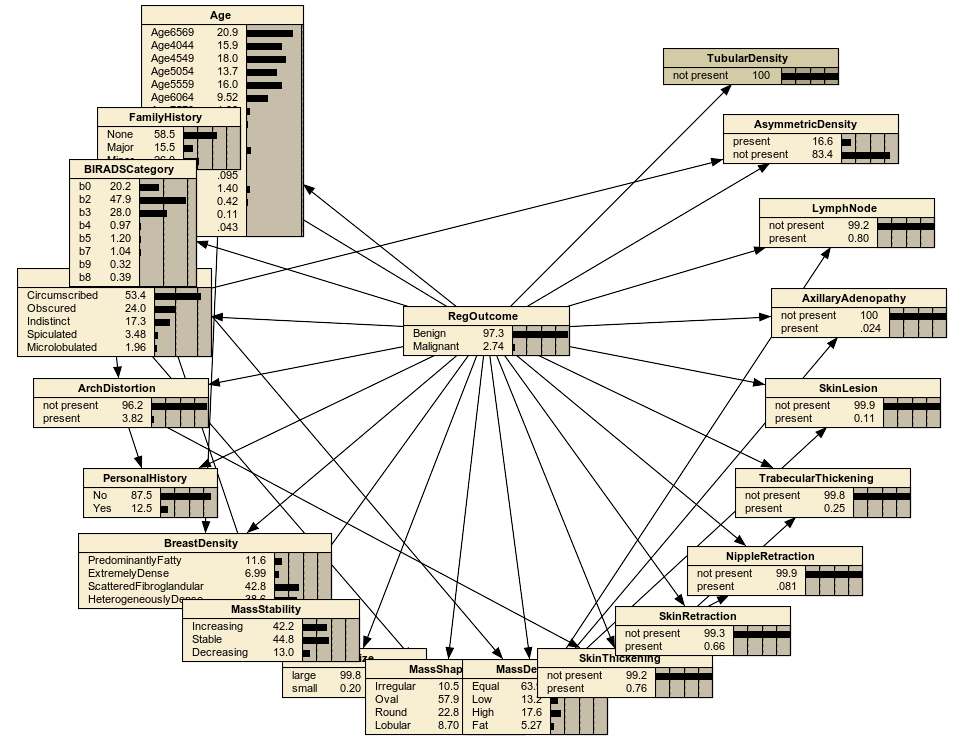
\includegraphics[width=\linewidth]{mass_net.png}
	\caption{The learned TAN model linking descriptors to malignancy}
	\label{fig:mass_net}
\end{figure}


\clearpage
\begin{figure}[h]
\centering
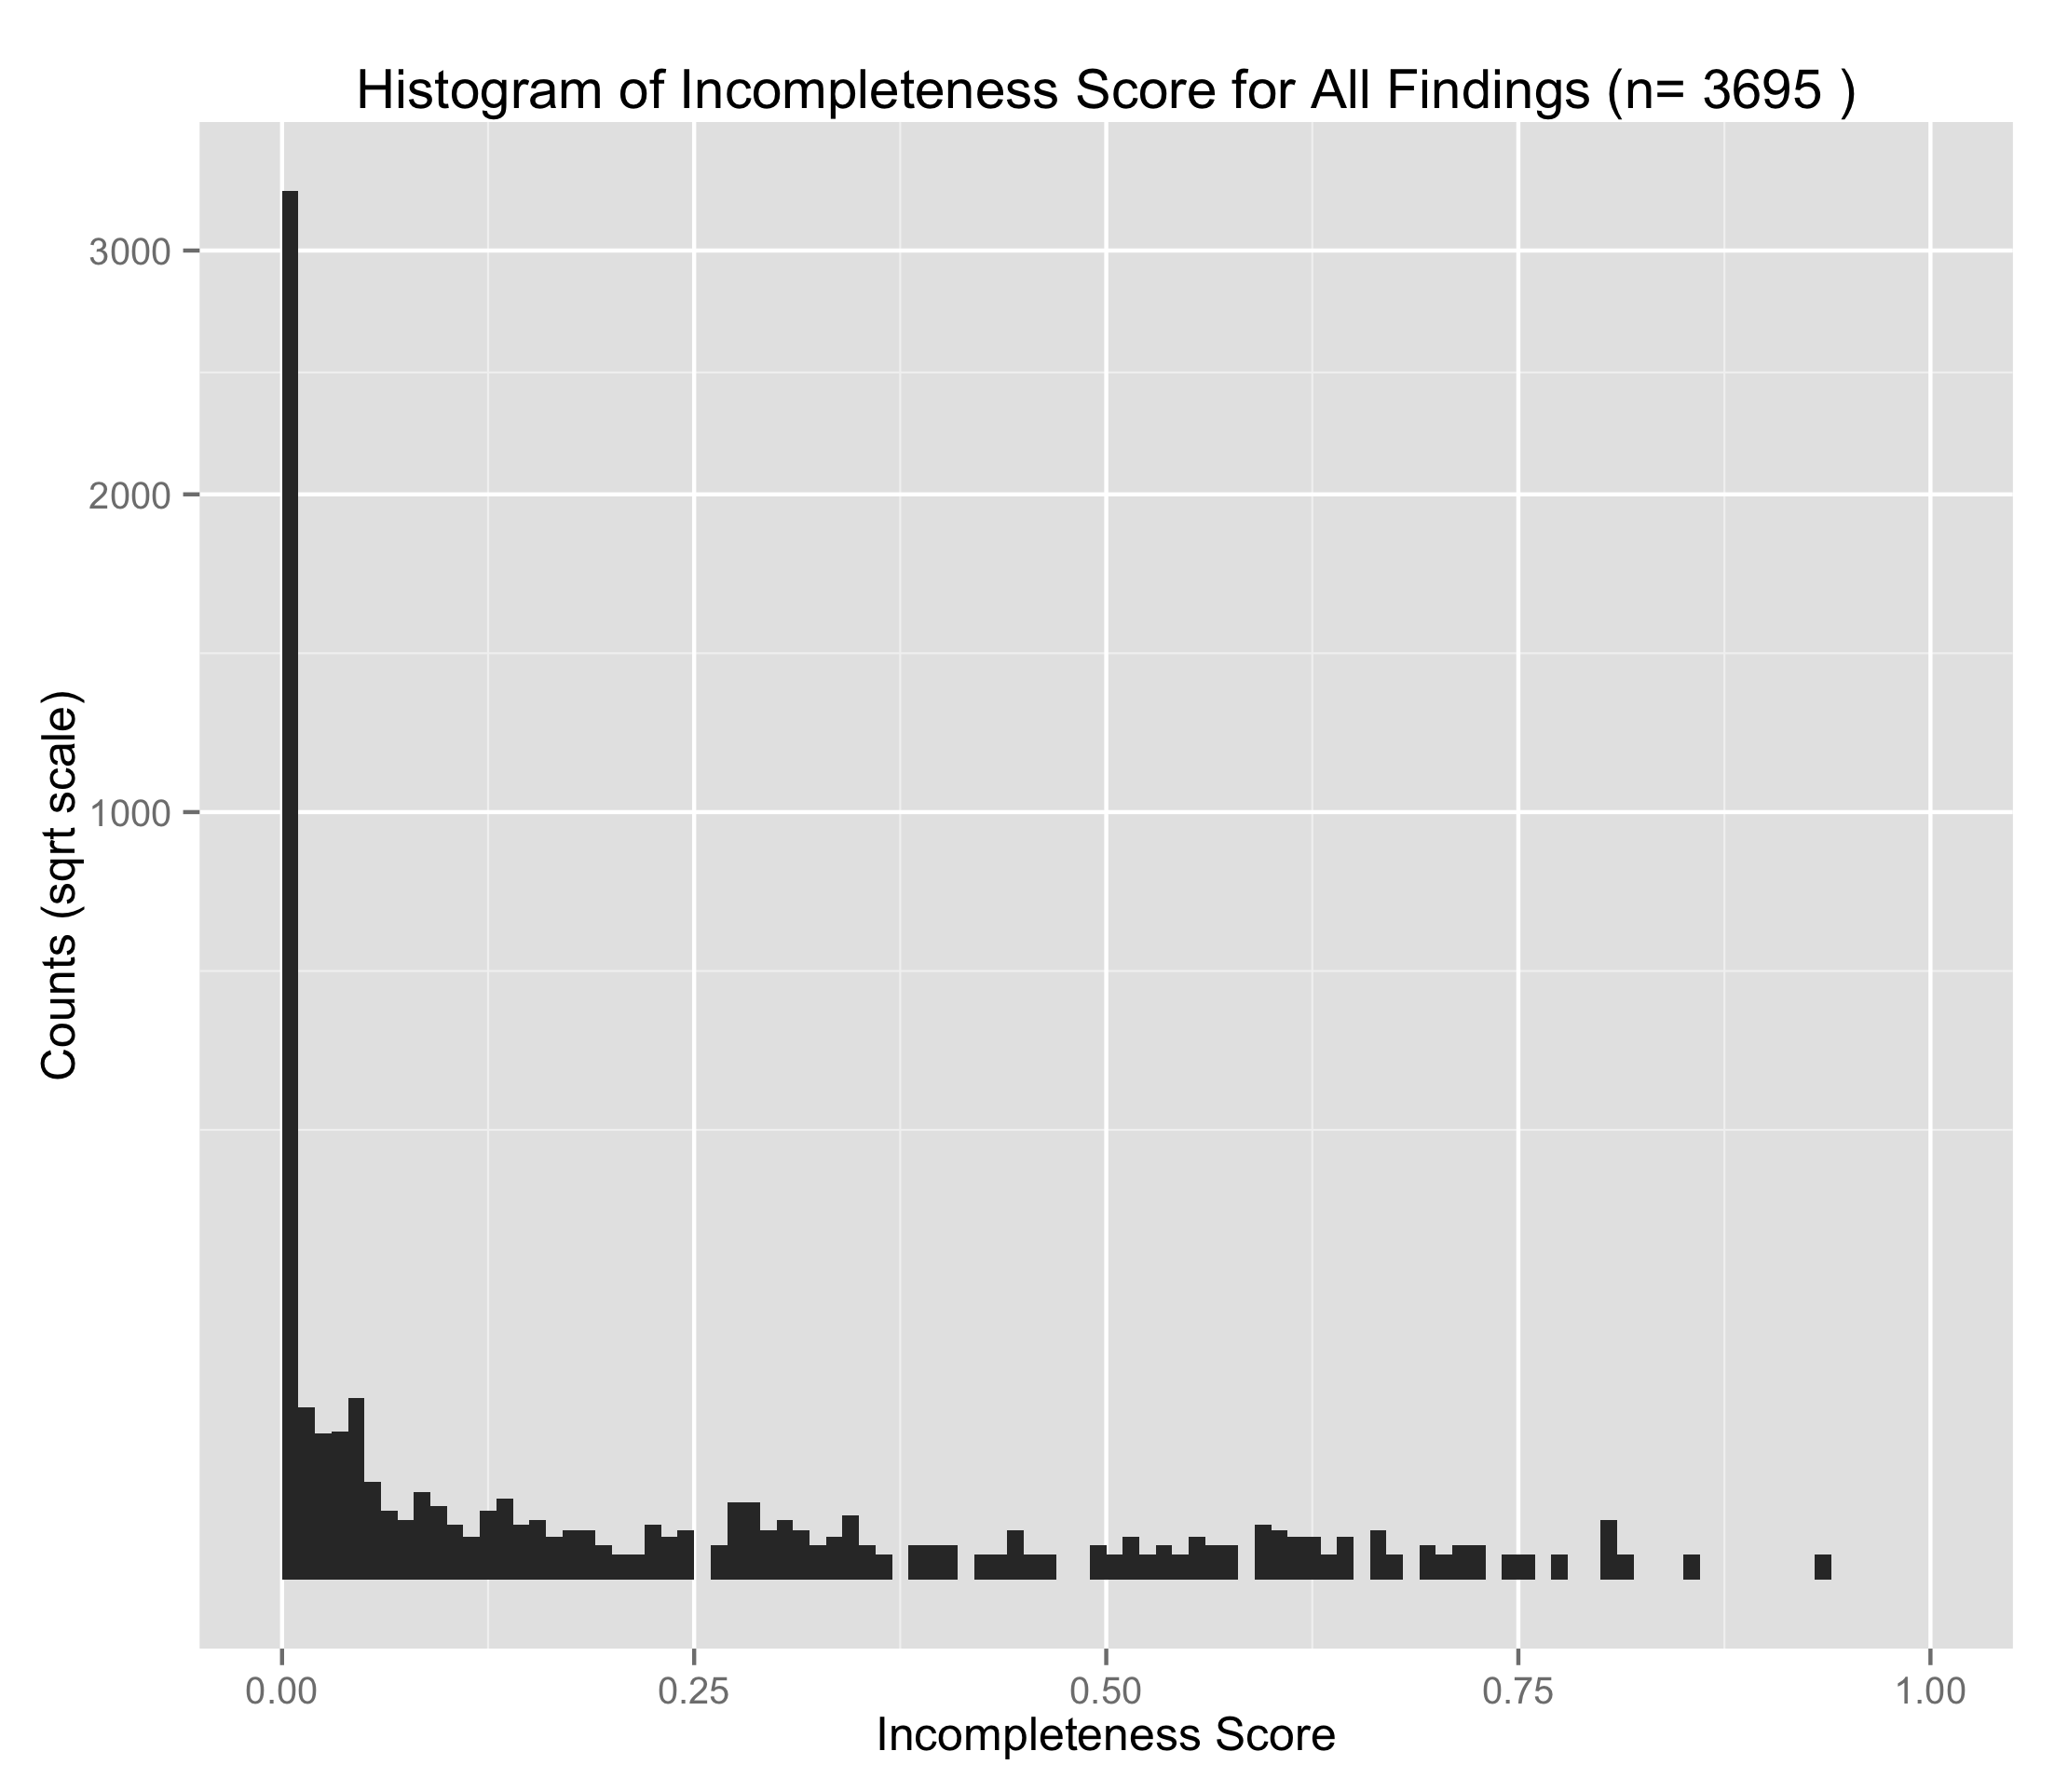
\includegraphics[width=\linewidth]{incompleteness_score_hist_all.png}
\caption{Histogram of all incompleteness scores in the test data set}
\label{fig:incompleteness_score_hist_all}
\end{figure}


\clearpage
In order to verify that the incompleteness score can be used to predict mammographic error, I plotted its histogram and density estimate stratified by radiological predictive categories: true negative (TN), false negative (FN), true positive (TP), and false positive (FP) [figure \ref{fig:incompleteness_score_hist_confmat}]. The graphs show that there are a large number of false positive and false negative cases that have non-zero incompleteness scores. Intuitively, this shows that incomplete reports have a higher likelihood of containing errors. The mean incompleteness score for erroneous cases ($FP \cup FN$) was \textbf{0.0720} while the mean incompleteness score for correct ($TP \cup TN$) cases was \textbf{0.0079}, an order of magnitude smaller. The difference between error and non-error incompleteness scores was statistically significant ($p < 2.2*10^{-16}$).

\begin{figure}[h]
\centering
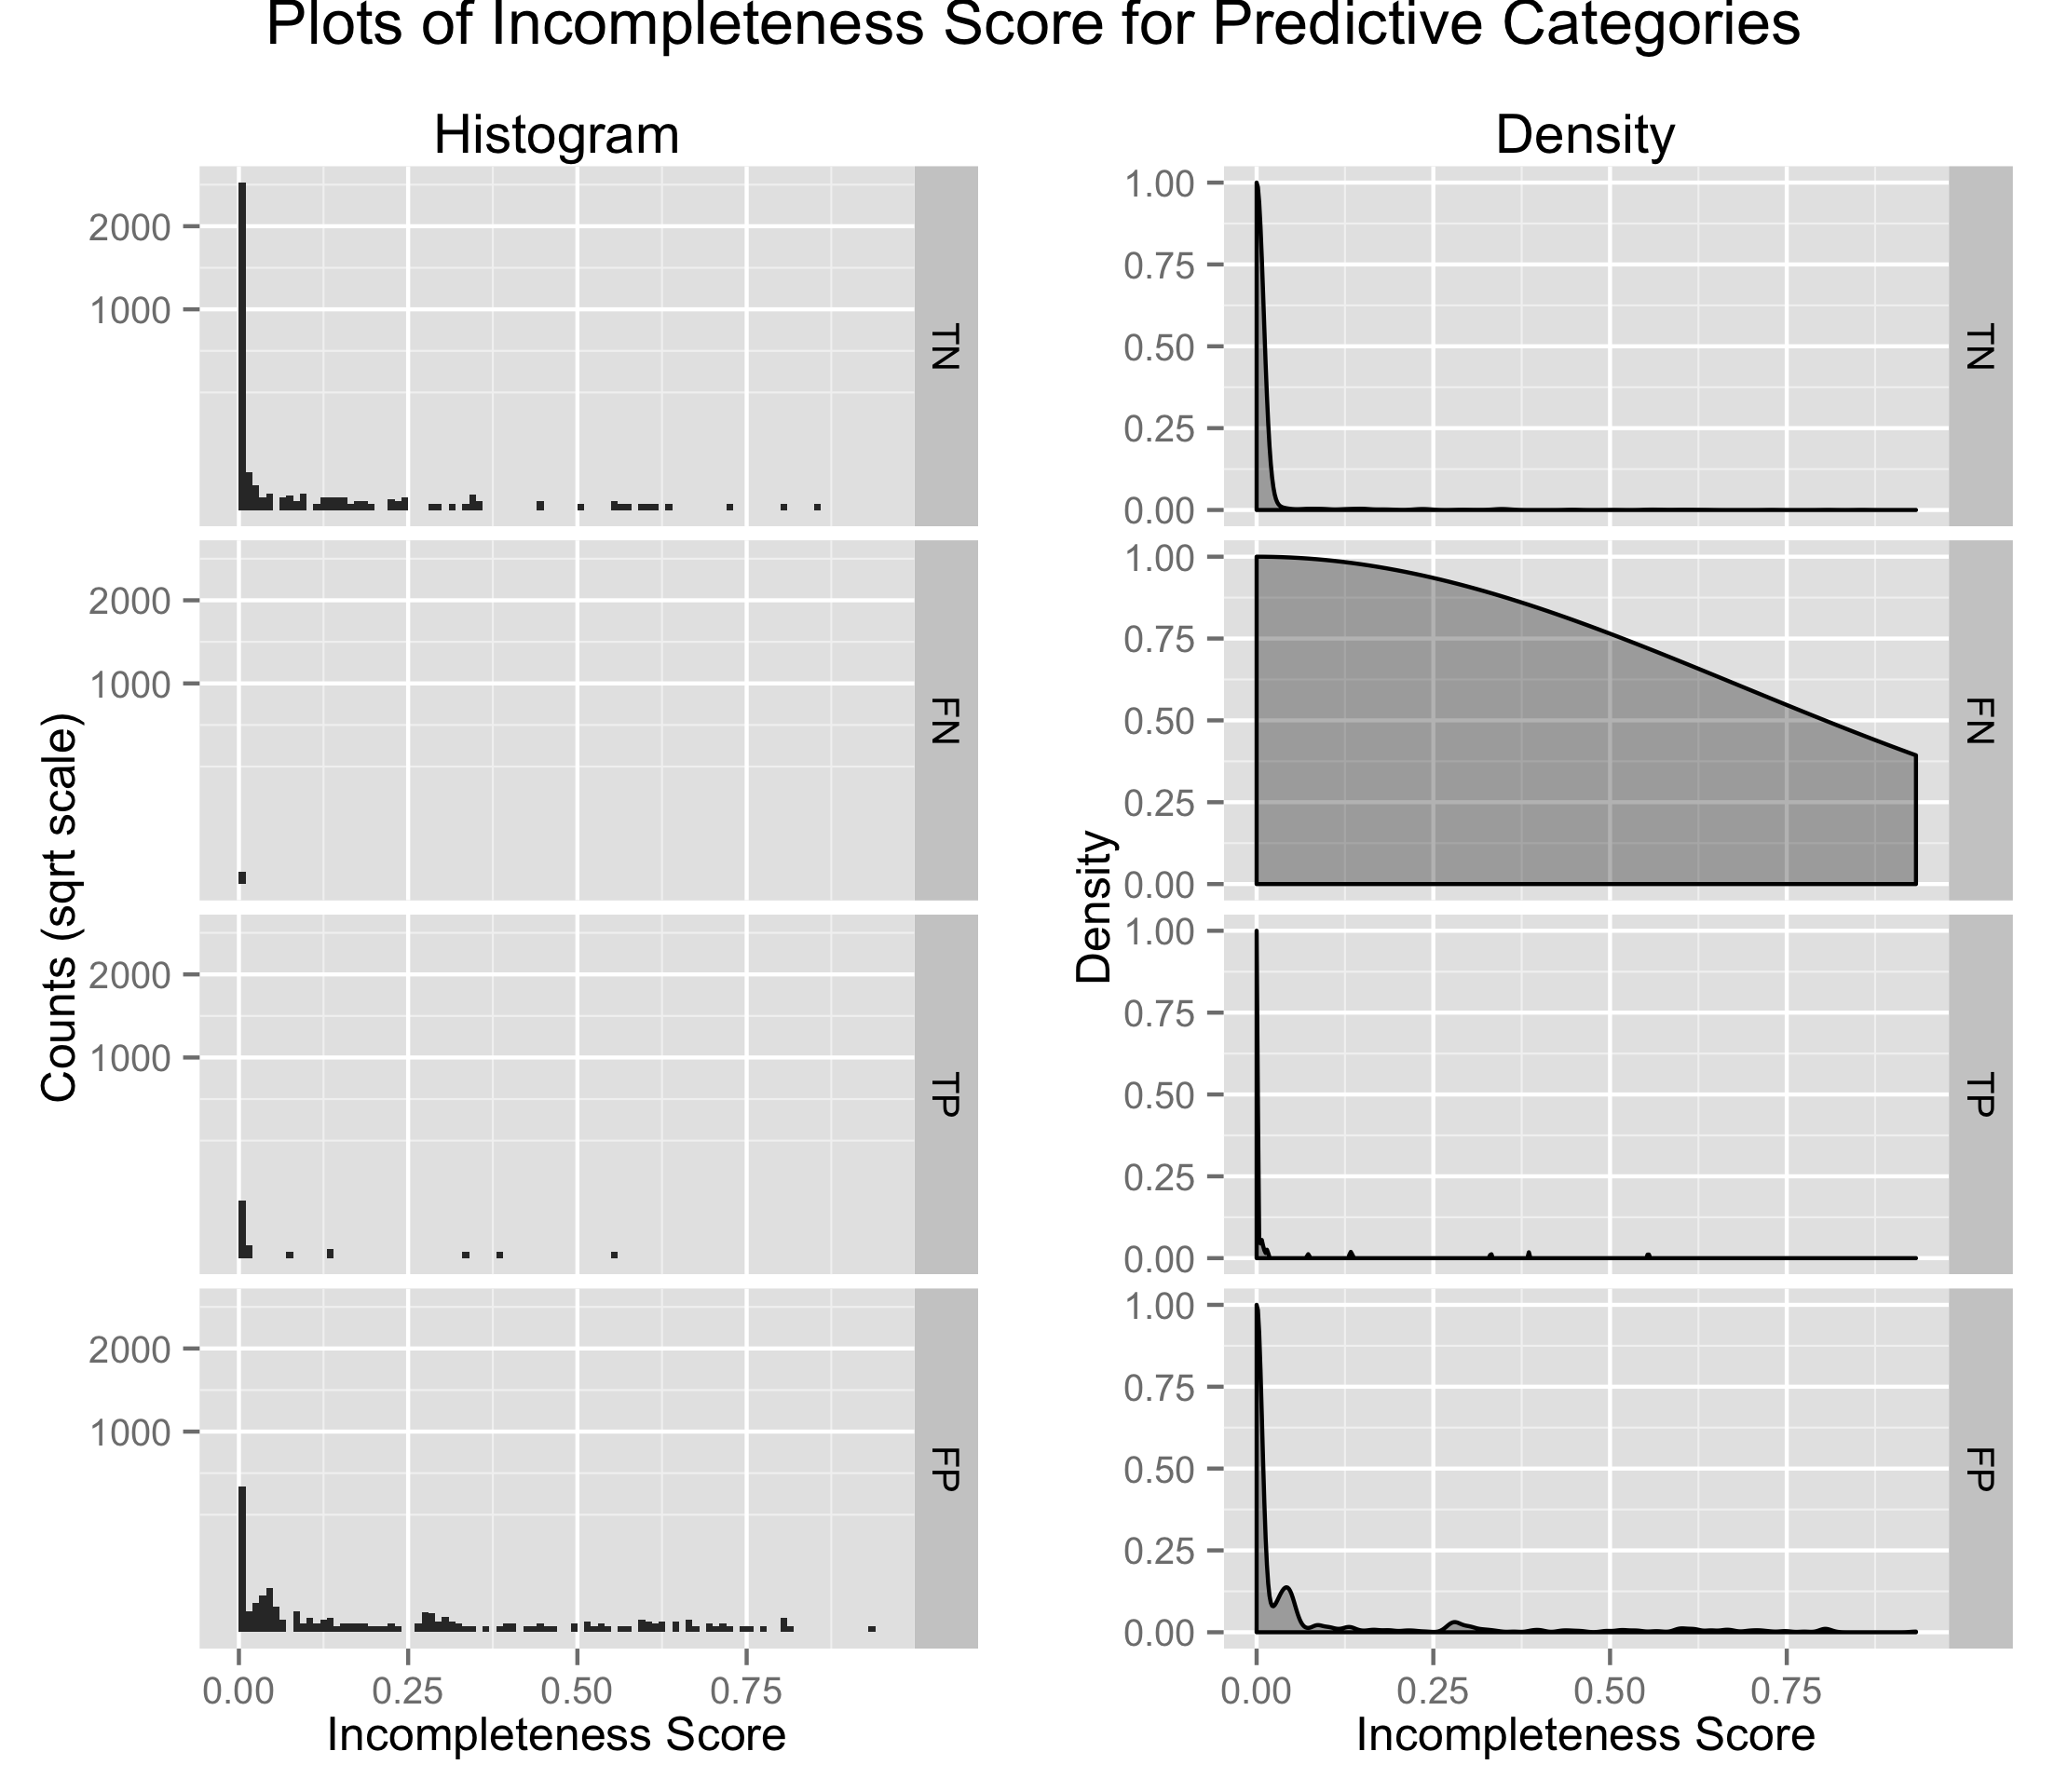
\includegraphics[width=\linewidth]{incompleteness_score_hist_confmat.png}
\caption[Incompleteness scores stratified by confusion matrix]{Plots of the histogram and density of incompleteness scores, stratified by radiologist performance on their respective cases. True Negative (TN) findings have the lowest incompleteness scores (indicating they are most complete) while false positive (FP) findings have higher incompleteness scores (indicating less completely reported findings). Joining (TN,TP) and (FP,FN), I can compare cases that were correctly assessed to cases with errors. Note that the false negative density graph has a nearly uniform distribution. This is an artifact due to the small amount of false negatives in the data set that skew density estimation.}
\label{fig:incompleteness_score_hist_confmat}
\end{figure}


An issue with this data is that there are a small number of false negative findings compared to false positive findings. This could skew results since positive findings may contain descriptors more prone to noise in the model. To account for this, I compared false positive to true positive results since both groups would have similar descriptors. The analysis showed that they were still statistically significantly different ($p<0.0026$).

\clearpage

I then tested how well the incompleteness score could predict error in mammography reading. Figure \ref{fig:incompleteness_rad_improvement} shows several performance metrics for different cutoffs of the incompleteness score. The maximal accuracy with respect to cutoffs was 0.826 at a cutoff of 0.018. This means that < 1.8\% probability of changing decisions when given new information should warrant describing more observations. The precision associated with this cutoff was 0.713 meaning 71.3\% of cases classified as errors via the incompleteness score with cutoff 0.018 will actually be errors. Finally, I measured the percentage reduction in total mammography error if each error marked for revision was corrected. Using the given cutoff, we saw a potential 21.7\% decrease in total errors.

\begin{figure}[h]
\centering
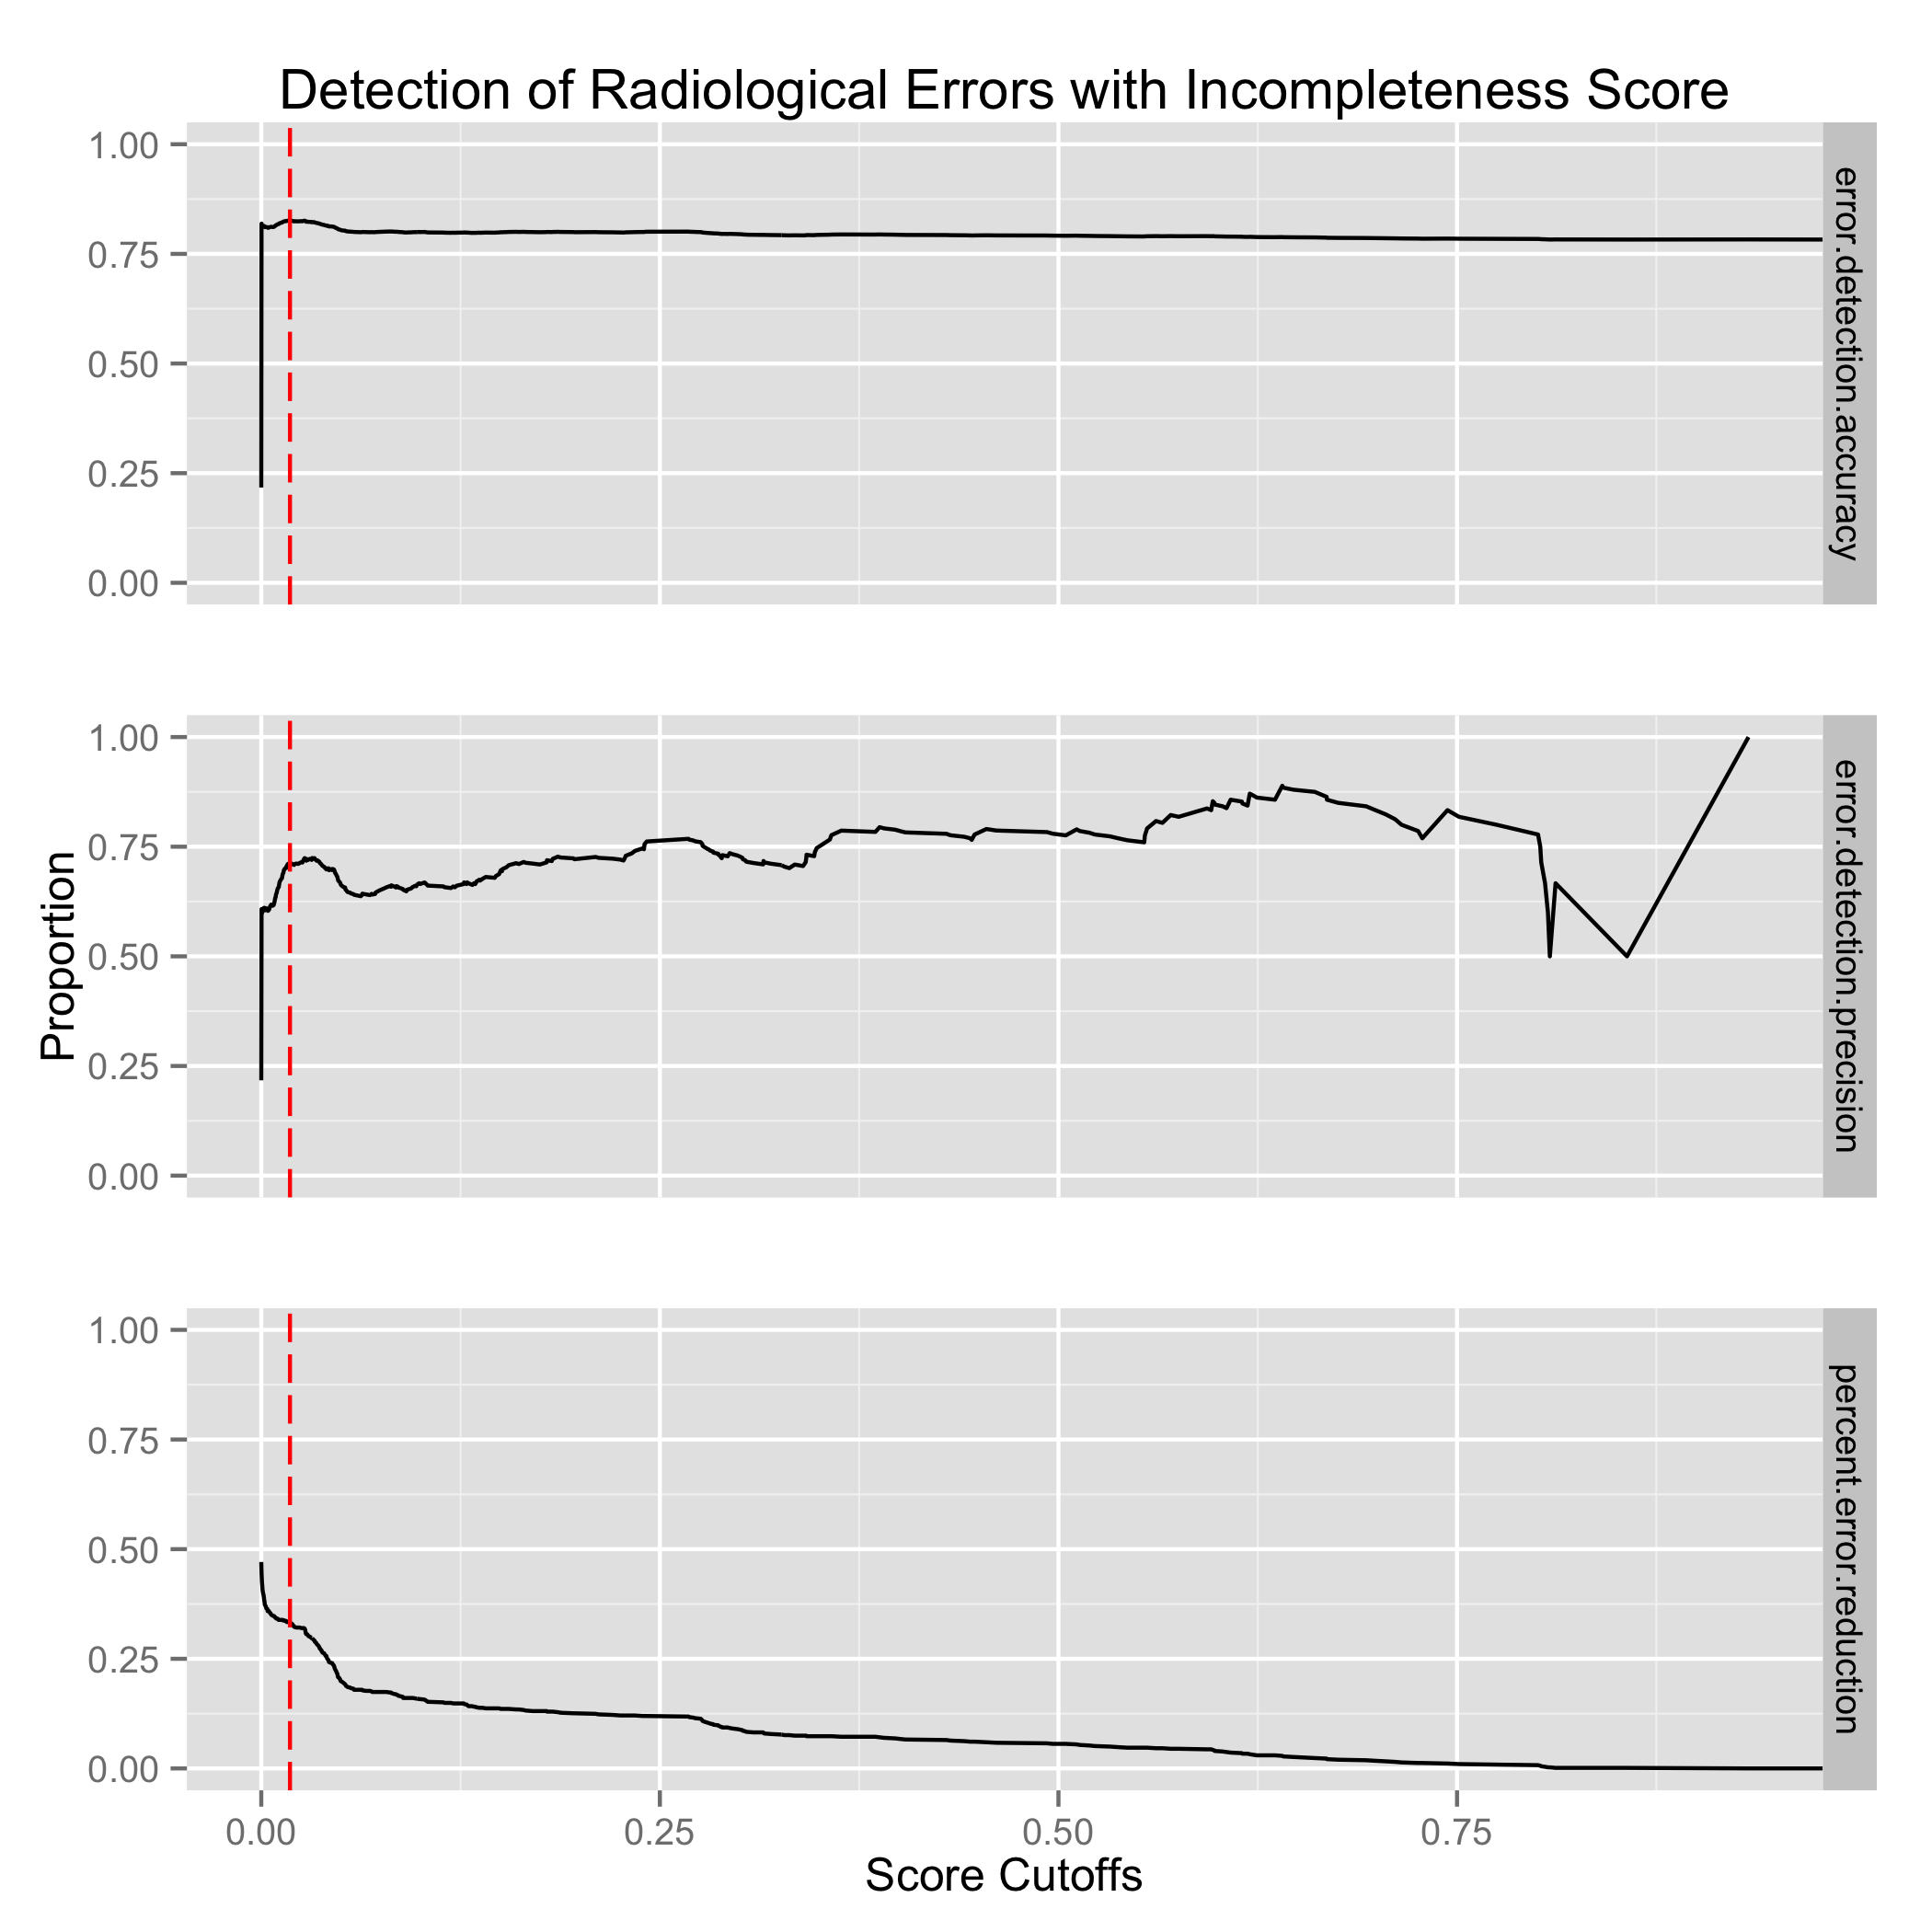
\includegraphics[width=\linewidth]{incompleteness_rad_improvement.png}
\caption[Radiological improvement with incompleteness scores]{Improvement in radiological performance for difference incompleteness cutoffs. First row shows the incompleteness score accuracy in predicting radiological errors. Second row shows incompleteness score positive predictive value in predicting error. Third row shows the percent reduction in error if identifying error at the specified cutoff. The red-dotted line shows the cutoff point that maximizes error classification accuracy (first panel).}
\label{fig:incompleteness_rad_improvement}
\end{figure}
